The size and complexity of modern software makes it almost impossible to avoid
implementation errors. Asynchronous computation, the rich array of computing
environments and their communication, and continuous modifications of source
code are among the challenges that can lead to software \enquote{going wrong}.

Prominent and costly examples of failure include the \ndx{Ariane 5} rocket
explosion on its maiden flight~\cite{ariane5}, the \ndx{Therac-25} radiation
therapy machine with six instances of lethal overdoses~\cite{leveson1993}; and
the loss of NASA's \ndx{Mars Climate Orbiter}~\cite{mars1999}.

In more recent memory, the \ndx{CrowdStrike} incident caused multiple days of
system outages across critical infrastructure like airports, banks, and
hospitals~\cite{crowdstrike}. In a case involving the~\textcite{usg2024}, a
software-related failure exposed sensitive personal information of USG employees
with potential harm to the Augusta University community.

Unreliability of software is not isolated to these few publicized instances.
A pithy comment in~\textcite[p. 3]{dijkstra1970} captures a similar sentiment.

\begin{quotation}
\noindent{}Present-day computers are amazing pieces of equipment, but most
amazing of all are the uncertain grounds on account of which we attach any
validity to their output.
\end{quotation}

The context of Dijkstra's statement is modest compared to exploding rockets. It
refers to the multiplication operation of two 27-bit integers. Checking that a
calculator actually performs the correct operation for all inputs---\ie meets
its \emph{specification\index{specifications}}---at a rate of few microseconds
per input-pair, would require more than 10,000 years. Thus, skepticism around
software correctness is a long-held position among some computer scientists. It
is also the core issue tackled by formal methods.

\paragraph*{Formal methods motivations and challenges.}
Formal methods aims to remove uncertainty by providing techniques that allow
establishing strong behavioral guarantees. Formal methods is deeply rooted in
mathematics and logic~\cite{shankar2023}. In this view, programs are defined as
precise mathematical \emph{models} with \ndx{specifications}. The specification
defines what behavior is expected from the model under study. Formally
\emph{verifying}\index{formal verification} a program involves constructing a
\emph{proof} that the model satisfies its specification. In contrast to manual
inspection and tests (like a test of inspecting every input-pair), a proof
conclusively ensures correctness for all inputs, at the model's level of
abstraction. As noted later by~\textcite{dijkstra1972}, \enquote{{[t]he only
effective way to raise the confidence level of a program significantly is to
give a convincing proof of its correctness.}}

The motivation for using formal methods is based on the strength of guarantees
it provides. Being formal helps when we want to be precise~\cite{leino2023}.
However, thinking formally requires a different engineering mindset. Instead of
thinking of all possible scenarios and how they might go wrong, formal reasoning
requires defining how a system is \emph{expected} to work, and identifying
conditions that must be met to ensure the correct behavior~\cite{aws2024}. Those
conditions are then formally verified with proofs.

Despite the clear benefits, wider adoption of formal methods still faces many
challenges. These include \eg resource investment (formal proofs are
time-consuming), tooling and tool maintenance, and technical
education~\cite{beek2024}. Another challenge concerns the \emph{methods}
themselves. The \ndx{Four Color theorem} is the first famous result with a proof
that requires large computer calculations. When the proof appeared in 2008, such
proofs were still controversial. The source of the controversy was that computer
programs could not be reviewed with mathematical rigor~\cite{gonthier2008}.
Thus, advancing formal methods also concerns improving communication about the
available capabilities.

\begin{quotation}
\noindent{}We can envision [\ldots] a world in which computer programs are
always the most reliable components of any system or device~\cite{hoare2021}.
\end{quotation}

\subsubsection{Foundational Concepts}
\label{subsubsec:verification-concepts}

\paragraph*{Formal models.} A formal \emph{model} is an abstract description of
a computer system of interest. The model is expressed in (some) formal modelling
language. The model is used for reasoning about the system and consequences of
design choices~\cite{zave2023,olveczky2017}. For the dissertation, the systems
of interest are programs.
In choosing a modeling formalism, it should enable expressing the model as
naturally and intuitively as possible, while still generating mathematically
precise structures~\cite{olveczky2017,beek2024}. In other words, the formalism
should
\begin{enumerate*}[label=(\roman*)]
\item omit unnecessary technicalities,
\item enable focusing on the problem of interest at an appropriate level of
abstraction, and
\item facilitate analysis and reasoning about the program~\cite{olveczky2017}.
\end{enumerate*}

\paragraph*{Specifications.} The \emph{specification}\index{specifications}
is a part of the formal model that describes the \emph{behavior} of the
program~\cite{zave2023b}. The specification should be simpler and easier to
comprehend than the implementation~\cite{zave2023b}. The development of the
specification should precede the implementation, or minimally be developed
concurrently~\cite{dijkstra1972}. Critically, we want the specification to be
{separate} from the implementation~\cite{furia2014b}. Independence isolates the
mathematical properties of interest and enables showing that the implementation
is consistent with those properties. Without independence, we encounter the
\emph{\ndx{Assertion Inference Paradox}}~\cite{furia2014b}. Essentially, the
paradox states: if we infer the specification from the implementation, what is
it that we prove?

\ndx{Hoare triple}s~\cite{hoare1969} are a standard way to express \ndx{specifications}.
In this view, we consider \(S\) to be some executable statement (a program).
We then define a \emph{\ndx{precondition}} \(P\)\symbo{pre} that describes conditions that hold before execution.
A \emph{\ndx{postcondition}} \(Q\)\symbo{post} describes conditions that hold after execution.
Then, a \emph{\ndx{Hoare triple}} is a predicate that connects the statement with the pre- and postconditions by \(\{P\} S \{Q\}\)\symbo{hoare}.
The expression means, \enquote{starting from \(P\)\symbo{pre}, statement \(S\) will not crash and terminates in a state satisfying \(Q\)\symbo{post}}.
For example, \(\{ \prm{x}=0 \}\;\prm{x++}\;\{\prm{x}=1\}\)\symbo{hoare} is a valid and provable \ndx{Hoare triple}.%
\footnote{The mechanics of how to prove it is a topic for~\autoref{subsubsec:sm-tool-examples}.}

\paragraph*{Invariants.}
Proving that an implementation meets its specification requires more information than what is available in the program syntax~\cite{chang2005}.
For example, to prove a Hoare triple of a loop command often requires establishing additional verification conditions.
An \emph{\ndx{invariant}}, in programming terms, is an assertion that is preserved by the program execution~\cite{furia2014}.
An invariant is \emph{inductive},
if it holds the first time a program location is reached and is preserved in every cycle returning to that location~\cite{sankaranarayanan2004}.
There are many kinds of invariants, \eg object, class, and loop invariants.
Although having invariants is useful for proving programs, discovering them is among the most difficult problems in verification~\cite{dillig2013,yu2023}.

To provide a concrete example, a \emph{loop invariant} is an expression that holds on loop entry and after every loop iteration.
The program of~\autoref{lst:invariant} has two variables, \pr|i| and \pr|n|.

\begin{center}
\begin{minipage}{\textwidth}
\captionsetup{type=lstlisting}
\cstarinputlisting{invariant.c}
\captionof{lstlisting}[Loop inspection for loop invariants]{Loop inspection for loop invariants.}
\label{lst:invariant}
\end{minipage}
\end{center}

At loop entry, the value of \pr|i| is 0.
If the value of \pr|n| is negative, the loop never iterates.
Otherwise, \pr|i| will hold a value between 0 and \pr|n|.
Based on this analysis, the loop invariant is \(0 \leq \prm{i} \leq \prm{n} \vee \prm{n} < 0\).
A postcondition of \pr|i| is \(\prm{i}=0 \vee \prm{i}=\prm{n}\).
A loop invariant is a {weakened} form of its postcondition~\cite{furia2010}.
Therefore, techniques that aim to infer invariants benefit from the availability of postconditions, as investigated in~\autoref{sec:postcond}.

Finally, a brief note about invariants and complexity.
It is possible to infer complexity bounds of numerical loops based on loop invariants as shown by~\textcite{nguyen2017}.
However, the solution relies on dynamic techniques, that are beyond purely static capabilities.

\paragraph*{Safety and \ndx{liveness properties}.}\index{safety properties}
Formal verification aims to guarantee that certain behavioral attributes, \ie \emph{properties}, hold for a program.
A few examples of properties are memory safety\ndx{memory safety}%
\footnote{\Ie absence of errors related to memory accesses: null-pointer de-referencing, access to un-allocated memory, dangling pointers, out-of-bounds accesses, double-free, \etc~\cite{muller2024}},
absence of overflows, termination, data race and \ndx{deadlock freedom}, secure \ndx{information flow} (cf~\autoref{if-security}), staying within available resource bounds, and \ndx{worst-case execution time} (WCET).
To show that a program is free of \eg overflows, we express {overflow-freedom} as a formal specification, then prove that the implementation satisfies the specification.

There are various different ways of categorizing classes of \ndx{properties}.
\emph{Functional} properties\index{properties!functional} are technical characteristics that contribute to computation of the correct output.
\emph{Non-functional} properties\index{properties!non-functional} are concerned with quality attributes like security, dependability, reliability, and resource requirements~\cite{terbeek2018}.
Two other frequently-used categorizing terms are safety and liveness.
They come from a paper by~\textcite{lamport1977}, where they are formulated as follows.
A \emph{\ndx{safety property}} is a guarantee that \enquote{something (bad) will not happen}.
A \emph{\ndx{liveness property}} ensures \enquote{(good) things must happen}, eventually.
The proof techniques across these safety and liveness properties are different.
The works in this dissertation are primarily concerned with non-functional safety properties.

\paragraph*{Partial and total correctness.}
Broadly, a program is correct if the implementation is consistent with the specification\index{specifications}~\cite{furia2014b}.
However, when making assertions about correctness, we need to be more precise.
There are two common notions about correctness that provide added specificity: partial and total correctness.
\emph{Partial correctness}\index{partial correctness} means that every terminating execution is correct, however it does not ensure every execution terminates~\cite[p. 64]{leino2023}.
A stronger guarantee follows from \ndx{total correctness}.
A program is \emph{totally correct} if it is partially correct and always terminates~\cite[p. 64]{leino2023}.
Total correctness can be viewed as a combination of safety\index{safety property} and liveness properties\index{liveness property}~\cite{lamport1977}.
There are several strategies for proving termination in some cases, \cf~\autoref{resource-analysis}.
However, a general method that proves termination of all programs cannot exist since termination is undecidable~\cite{turing1936}\index{undecidability}.
This means it is impossible to show \ndx{total correctness} of all programs.%
\footnote{Total correctness is not always ideal.
There are many applications where termination is undesirable, like a web server and cardiac pacemaker, but where we still want formal guarantees.};
However, similar to~\autoref{static-analysis-basics}, there is endless opportunity in building increasingly more capable program verifiers.

\subsubsection{Tools for Formal Verification}

Formal methods is inherently concerned with \emph{computer-aided} reasoning.
Therefore, software tools are essential to formal methods. The tools include
solvers, theorem provers, model checkers, verifiers, \etc. Each tool family has
different use cases, degree of automation, and guarantees -- as illustrated
in~\autoref{fig:verification-approaches}, adapted from~\textcite{leroy2018}.

\begin{figure}[ht]
\centering
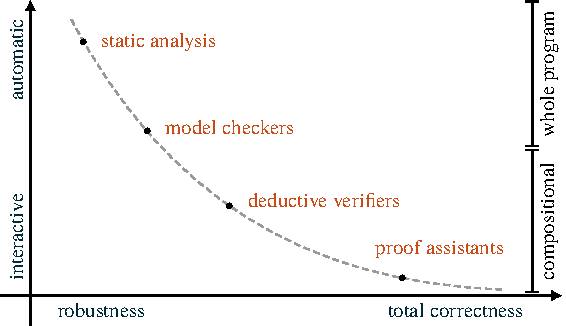
\includegraphics[]{fig_fm-tools}
\caption[Formal verification approaches]{
Formal verification approaches.}
\label{fig:verification-approaches}
\end{figure}

\autoref{tab:fm-tools} provides a directory of specific formal methods tools.
Interactive theorem provers and verification-aware programming languages are of
special interest to this dissertation.

\begin{table}[p!]
\begin{tabularx}{\linewidth}{@{}lX@{}}
\toprule
\multicolumn{2}{@{}l}{\textbf{Automated theorem provers \& solvers}} \\
&
\href{https://alt-ergo.ocamlpro.com}{\ndx{Alt-Ergo}}%
,{ }\href{https://github.com/bitwuzla/bitwuzla}{\ndx{Bitwuzla}}%
,{ }\href{https://cvc5.github.io}{\ndx{cvc5}}%
,{ }\href{https://www.cyclist-prover.org}{\ndx{Cyclist}}%
,{ }\href{https://github.com/dreal/dreal4}{\ndx{dReal}}%
,{ }\href{https://wwwlehre.dhbw-stuttgart.de/~sschulz/E/E.html}{\ndx{E}}%
,{ }\href{https://gitlab.com/korovin/iprover}{\ndx{iProver}}%
,{ }\href{https://mathsat.fbk.eu}{\ndx{MathSAT}}%
,{ }\href{https://fmv.jku.at/picosat/}{\ndx{PicoSAT}}%
,{ }\href{https://github.com/uuverifiers/princess}{\ndx{Princess}}%
,{ }\href{https://en.wikipedia.org/wiki/Prover9}{\ndx{Prover9}}%
,{ }\href{https://satallaxprover.org}{\mbox{\ndx{Satallax}}}%
,{ }\href{https://www.mpi-inf.mpg.de/departments/automation-of-logic/software/spass-workbench/}{\ndx{SPASS}}%
,{ }\href{https://vprover.github.io}{\ndx{Vampire}}%
,{ }\href{https://verit.loria.fr}{\ndx{veriT}}%
,{ }\href{https://yices.csl.sri.com}{\ndx{Yices}}%
,{ }\href{https://github.com/Z3Prover/z3}{\ndx{Z3}}%
\\\midrule
\multicolumn{2}{@{}l}{\textbf{Interactive theorem proving}} \\
&
\href{https://github.com/agda/agda}{\ndx{Agda}}%
,{ }\href{https://github.com/EasyCrypt/easycrypt}{\ndx{EasyCrypt}}%
,{ }\href{https://fstar-lang.org}{\ndx{F$^{*}$}}%
,{ }\href{https://hol-light.github.io}{\ndx{HOL Light}}%
,{ }\href{https://iris-project.org}{\ndx{Iris}}%
,{ }\href{https://isabelle.in.tum.de}{\ndx{Isabelle}}%
,{ }\href{https://lean-lang.org}{\ndx{Lean}}%
,{ }\href{https://us.metamath.org}{\ndx{Metamath}}%
,{ }\href{https://en.wikipedia.org/wiki/Mizar_system}{\ndx{Mizar}}%
,{ }\href{https://pvs.csl.sri.com}{\ndx{PVS}}%
,{ }\href{https://rocq-prover.org}{\ndx{Rocq}}%
,{ }\href{https://github.com/boyland/sasylf}{\ndx{SASyLF}}%
,{ }\href{https://github.com/ggrov/tinker}{\ndx{Tinker}}%
\\\midrule
\multicolumn{2}{@{}l}{\textbf{Invariant synthesis}} \\
&
\href{https://github.com/PL-ML/code2inv}{Code2Inv}\index{Code2Inv}%
,{ }\href{https://plse.cs.washington.edu/daikon/}{Daikon}\index{Daikon}%
,{ }\href{https://github.com/dynaroars/dig/tree/dev}{DIG}\index{DIG}%
,{ }\href{https://github.com/freqhorn/freqhorn}{FreqHorn}\index{FreqHorn}%
\\\midrule
\multicolumn{2}{@{}l}{\textbf{Language-based verification \& modelling languages}} \\
&
\href{https://github.com/boogie-org/boogie}{Boogie}\index{Boogie}%
,{ }\href{https://dafny.org}{Dafny}\index{Dafny}%
,{ }\href{https://www.eiffel.org}{Eiffel}\index{Eiffel}%
,{ }\href{https://cs.nyu.edu/~wies/software/grasshopper/}{GRASShopper}\index{GRASShopper}%
,{ }\href{https://kframework.org}{K}\index{K Framework}%
,{ }\href{https://en.wikipedia.org/wiki/Maude_system}{Maude}\index{Maude}%
,{ }\href{https://rebeca-lang.org}{Rebeca}\index{Rebeca}%
,{ }\href{https://en.wikipedia.org/wiki/SPARK_(programming_language)}{SPARK}\index{SPARK}%
,{ }\href{https://en.wikipedia.org/wiki/TLA+}{TLA+}\index{TLA+}%
,{ }\href{https://github.com/utwente-fmt/vercors}{VerCors}\index{VerCors}%
,{ }\href{https://www.pm.inf.ethz.ch/research/viper.html}{Viper}\index{Viper}%
,{ }\href{https://whiley.org}{Whiley}\index{Whiley}%
,{ }\href{https://www.why3.org}{Why3}\index{Why3}%
\\\midrule
\multicolumn{2}{@{}l}{\textbf{Language extensions adding verification features}} \\
&
\href{https://en.wikipedia.org/wiki/ACL2}{ACL2}\index{ACL2}% %(Common LISP),
,{ }\href{https://www.atelierb.eu/en/atelier-b-tools/online-documentation/}{Atelier B}\index{Atelier B}%
,{ }\href{https://github.com/ocaml-gospel/cameleer}{Cameleer}\index{Cameleer}% %(Ocaml),
,{ }\href{https://github.com/flux-rs/flux}{Flux}\index{Flux}% %(Rust),
,{ }\href{https://frama-c.com}{Frama-C}\index{Frama-C}% %(C),
,{ }\href{https://github.com/viperproject/gobra}{Gobra}\index{Gobra}% %(Go),
,{ }\href{https://www.key-project.org/applications/program-verification/}{KeY}\index{KeY}% %(Java),
,{ }\href{https://ucsd-progsys.github.io/liquidhaskell/}{LiquidHaskell}\index{LiquidHaskell}% %(Haskell),
,{ }\href{https://github.com/marcoeilers/nagini}{Nagini}\index{Nagini}% %(Python),
,{ }\href{https://www.openjml.org}{\mbox{OpenJML}}\index{OpenJML}% %(Java),
,{ }\href{https://github.com/viperproject/prusti-dev}{Prusti}\index{Prusti}% %(Rust),
,{ }\href{https://github.com/epfl-lara/stainless}{\mbox{Stainless}}\index{Stainless}% %(Scala),
,{ }\href{https://github.com/verifast/verifast}{VeriFast}\index{VeriFast}% %(C, Rust, Java)
\\\midrule
\multicolumn{2}{@{}l}{\textbf{(Mixed Integer) Linear programming \& optimization}} \\
&
\href{https://github.com/coin-or/Clp}{Clp}\index{Clp}%
,{ }\href{https://en.wikipedia.org/wiki/CPLEX}{CPLEX}\index{CPLEX}%
,{ }\href{https://developers.google.com/optimization/cp/cp_solver}{CP-SAT}\index{CP-SAT}%
,{ }\href{https://github.com/COPT-Public/cuPDLP-C}{cuPDLP-C}\index{cuPDLP-C}%
,{ }\href{https://en.wikipedia.org/wiki/GLOP}{Glop}\index{Glop}%
,{ }\href{https://www.gnu.org/software/glpk/}{GLPK}\index{GLPK}%
,{ }\href{https://en.wikipedia.org/wiki/Gurobi_Optimizer}{Gurobi}\index{Gurobi}%
,{ }\href{https://github.com/ERGO-Code/HiGHS}{HiGHS}\index{HiGHS}%
,{ }\href{https://sat4j.org}{Sat4j}\index{Sat4j}%
\\\midrule
\multicolumn{2}{@{}l}{\textbf{Model checking}} \\
&
\href{https://alloytools.org}{Alloy}\index{Alloy}%
,{ }\href{https://github.com/moves-rwth/attestor}{\ndx{Attestor}}%
,{ }\href{https://vsl.cis.udel.edu/trac/civl/wiki}{\ndx{CIVL}}%
,{ }\href{https://cpachecker.sosy-lab.org}{\ndx{CPAChecker}}%
,{ }\href{https://github.com/diffblue/cbmc}{\ndx{CProver}}%
,{ }\href{https://github.com/uuverifiers/eldarica}{\ndx{Eldarica}}%
,{ }\href{https://github.com/loonwerks/jkind}{\ndx{JKind}}%
,{ }\href{https://github.com/nidhugg/nidhugg}{\ndx{Nidhugg}}%
,{ }\href{https://www.prismmodelchecker.org}{\ndx{PRISM}}%
,{ }\href{https://rebeca-lang.org/alltools/RMC}{\ndx{RMC}}%
,{ }\href{https://sri-csl.github.io/sally/}{\ndx{Sally}}%
,{ }\href{https://github.com/tlaplus/tlaplus}{\ndx{TLC}}%
,{ }\href{https://uppaal.org}{\mbox{\ndx{UPPAAL}}}%
\\\midrule
\multicolumn{2}{@{}l}{\textbf{Symbolic execution}} \\
&
\href{https://github.com/jburnim/crest}{\ndx{CREST}}%
,{ }\href{https://github.com/pschanely/CrossHair}{\ndx{CrossHair}}%
,{ }\href{https://github.com/GillianPlatform/Gillian}{\ndx{Gillian}}%
,{ }\href{https://klee-se.org}{\ndx{KLEE}}%
,{ }\href{https://github.com/runtimeverification/kontrol}{\ndx{Kontrol}}%
,{ }\href{https://github.com/OCamlPro/owi}{\ndx{owi}}%
,{ }\href{https://github.com/SymbolicPathFinder/jpf-symbc}{\ndx{Symbolic JPF}}
\\
\bottomrule
\caption[Tools for formal methods]{A categorized collection of formal methods tools.}
\label{tab:fm-tools}
\end{tabularx}
\end{table}

\begin{description}
\item[Mechanized proofs.]
One of the main goals of formal methods is to produce mechanized, \ie machine-checked, proofs.
A mechanized proof \enquote{detaches} proof-checking from the activity of crafting the proof.
Only the interface of the program, \ie the statement of the theorem, needs to be reviewed.
The rest is self-checking and deferred to a theorem prover.
This means everyone with sufficient technical abilities can check the proof once a proof exists (provided they trust the theorem prover).
Mechanized proofs are sometimes compared to \emph{paper proofs}, \ie informal proofs written in natural language, whether actually on paper or written in a text editor.
Since paper proof rely solely on the readers abilities to comprehend and confirm the detailed proof steps, mechanized proofs are functionally distinct and provide more rigorous correctness guarantees~\cite{gonthier2008}.

\item[Theorem provers.]

Mechanized (formal) proofs are created with theorem provers.
There are broadly two categories.

   \begin{itemize}
   \item An \emph{automatic theorem prover} (ATP) aims to find proofs without assistance from a user.
   The proof \emph{search} problem is challenging.%
   \footnote{\Eg for first-order logic, the problem is NP-complete~\cite{cook1971, levin1973})}%
   However, the solvers must be practically efficient to support various applications of automated theorem proving.
   Prominent ATPs complete bi-annually on solving \href{https://www.tptp.org}{\enquote{Thousands of Problems for Theorem Provers}} (TPTP problems)~\cite{sutcliffe2024} at the \href{https://tptp.org/CASC/}{CADE ATP System Competition} (CASC) -- the world championship for automated theorem proving~\cite{casc}.

   \item An \emph{interactive theorem prover} (ITP), \aka \emph{proof assistant}, is a programming environment that helps users write mechanized proofs.
   Proof assistants vary in underlying logics and proof style.
   To provide some metric of comparability, there is a ranking for tracking the formalization extent of 100 well-known mathematical theorems across proof assistants.
   As of April 2025, the top 3 proof assistants with highest coverage of the problems are Isabelle (92\%), HOL Light (89\%), and Rocq (79\%)~\cite{hundredtheorems}.
   \end{itemize}

While automatic theorem provers search for proofs of isolated problems and frequently serve as building block of other verification tools,
interactive theorem provers enable large and complex modular proof developments.

\item[Verification-aware programming languages.]
Verification-aware programming languages provide a conceptually different approach to machine-checked proofs.
Such languages are particularly well-suited for reasoning about functional correctness of programs.
Verification-aware programming languages have built-in capabilities to express specifications and proofs.
Additionally, they have an associated verifier that checks the proofs during program development;
typically, a background ATP that offers an interaction interface via a programming language~\cite{leino2023}.
One prominent style among the verification-aware languages is \emph{deductive verification},
where the verification process is based on some form of logical inference, i.e., \enquote{deduction}.
The properties to be proven are expressed in a formal specification language, as structured comments, next to the program constructs they relate to~\cite{hahnle2019}.
A deductive verifier them aims at to prove that all possible behaviors of a program satisfy the specification using the available program annotations~\cite{cassez2022}.
\end{description}

The remainder of this section briefly introduces two tools for formal methods:
the (interactive) \ndx{Rocq} theorem prover (\autoref{subsec:rocq}) and the
verification-aware programming language \ndx{Dafny} (\autoref{subsec:dafny}).
These tools are relevant for some of the dissertation manuscripts and assumed to
be familiar to the reader.

\subsubsection{The Rocq Theorem Prover}
\label{subsec:rocq}

The \ndx{Rocq} theorem prover is an interactive proof assistant for machine-checked formal reasoning.
It provides a rich and flexible environment for various proof developments.
\ndx{Rocq} is a widely-adopted tool in the programming languages research community, with applications in formal assurance of mathematics, semantics, and verification.
In 2013, The ACM has recognized Rocq with the
\href{https://awards.acm.org/software-system}{\ndx{Software System Award}} --
the highest distinction awarded to research software~\cite{rocq-community}.
The success of \ndx{Rocq} has also created abundant interest in \ndx{dependent type theory},
which is the core logic of \ndx{Rocq}~\cite{coquand1988}.

\paragraph*{Technical overview.}
As a guiding example, consider simple proof in~\autoref{lst:rocq-basic}.
The \pr|lemma| keywords starts a statement we wish to prove.
The specification language for stating theorems is called Gallina.
The code between \pr|Proof| and \pr|Qed| is a \emph{proof script}.
Proof scripts consists of \emph{tactics}.
Tactics perform operations on the proof state and make explicit the steps needed to prove the associate lemma.
The Rocq prover comes with dozens of built-in tactics.
In the example, \pr|intros|, \pr|simpl| and \pr|reflexivity| are tactics.
The tactic language is called Ltac.

\begin{center}
\begin{minipage}{\textwidth}
\captionsetup{type=lstlisting}
\rocqinputlisting{example.v}
\captionof{lstlisting}[A simple proof in Rocq]{A simple proof in Rocq.}
\label{lst:rocq-basic}
\end{minipage}
\end{center}

Proof engineers write proof scripts incrementally.
At each step, marked with a period, it is possible to evaluate the proof and see what goal should be proved next.
Refer to \autoref{fig:rocq-use} for a visual.
In the editor, the goal appears visually as a \emph{proof state}.

A full-fledged proof development consists roughly of definitions, lemmas, and proofs.
Definitions describe all the abstract structures we want to reason about in the mechanization,
and lemmas\footnote{The distinction between a lemma, theorem, corollary, \etc, is just syntactic sugar.}
prove facts about the structures.
Definitions and lemmas provide the specification of a proof development.
Formal verification then reduces to discovering the proofs that show that the specification is satisfied.
A finished proof is machine-checkable to everyone familiar with these technical basics.
Programs proved in Rocq can be extracted to other target languages.
The functional languages currently available as output languages are
OCaml, Haskell and Scheme~\cite{rocqdoc}.

\begin{figure}[ht]
\begin{center}
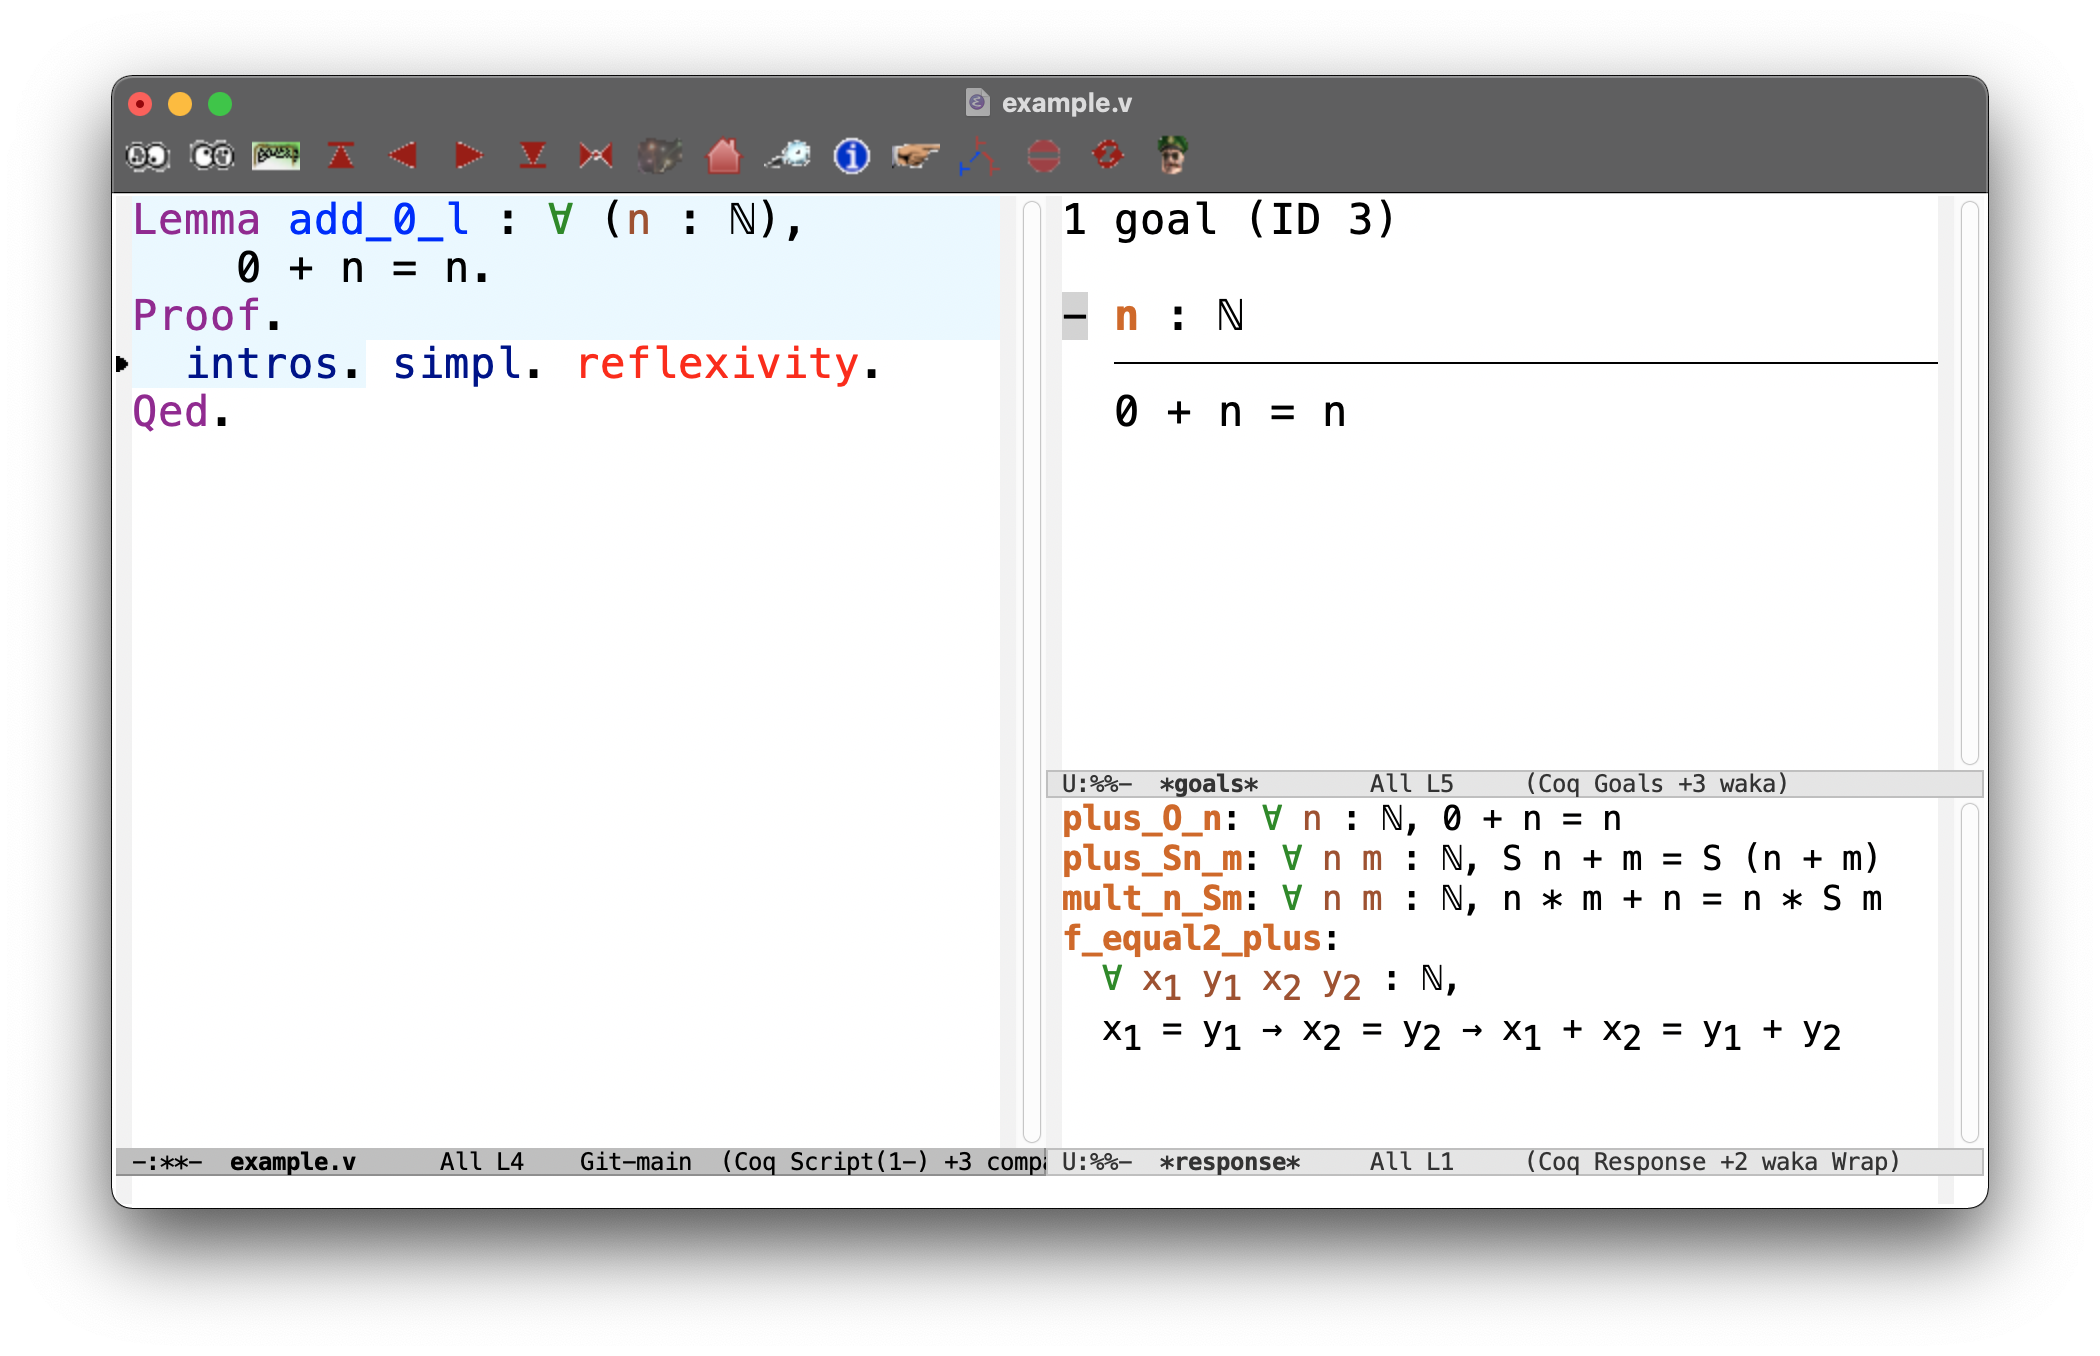
\includegraphics[width=.9\textwidth]{fig_ide}
\end{center}
\caption[Development view of the simple Rocq proof]
{A development view of the simple Rocq proof.
The Emacs editor is enhanced with the \href{https://proofgeneral.github.io/}{Proof General} interface
and the \href{https://github.com/cpitclaudel/company-coq}{Company-coq} plug-in.
The left view contains the proof code under development.
Focusing between \pr|Proof| and \pr|Qed| activates the {proof mode}.
While in proof mode, the {proof state} is visible in the top-right view.
The bottom-right view shows search results that appear after a database lookup for existing related lemmas.}
\label{fig:rocq-use}
\end{figure}

\paragraph*{Mathematical Components.}
The Mathematical Components library---colloquially mathcomp---extends the Rocq ecosystem with an extensive and coherent collection of formalized mathematical theories.
The library covers a wide spectrum of topics, including formal theory of general purpose data structures like lists;
prime numbers and finite graphs, and advanced topics in algebra.
The theories are organized into hierarchical levels where the design facilitates reuse.
The proof style is based on Rocq, but Mathematical Components uses a specialized language extension called SSReflect (small-scale reflection).
SSReflect significantly influences proof writing style and poses its own learning curve.
To demonstrate the difference,~\autoref{subsubsec:sm-tool-examples} shows examples in \enquote{standard} Rocq and SSReflect.
The Mathematical Components library has an essential role in the Rocq community because several landmark results of finite group theory are based on it.
For example, the mechanical proofs of the Four Colour theorem~\cite{gonthier2008} and the Odd Order theorem~\cite{gonthier2013} utilize the library extensively.

\paragraph*{Demonstrated applications.}
Conventional uses of Rocq include proving properties of programming languages, formalizing mathematics, and teaching.
\autoref{tab:rocq-results} contains representative examples across the first two categories.

\begin{table}
%! suppress = EscapeAmpersand
\begin{NiceTabularX}{\textwidth}{@{}l@{ }X@{}}
   \toprule
   \textbf{Formalization target} & \textbf{Authors} \\
   \midrule
   \href{https://users.dimi.uniud.it/~ivan.scagnetto/pi-calculus.html}%
   {\ndx{\(\pi\)-calculus} in (Co)inductive-type theory}\index{coinduction}
   & \textcite{honsell2001}
   \\
   \href{https://github.com/rocq-community/goedel}%
   {\ndx{Gödel-Rosser incompleteness theorem}}
   & \textcite{oconnor2005}
   \\
   Modal model of impredicative semantics
   & \textcite{appel2007}
   \\
   \href{https://github.com/rocq-community/fourcolor}%
   {\ndx{Four Color theorem}}%
   \smtabularnote{based on~\cite{robertson1997} and~\cite{appel1989}}
   & \textcite{gonthier2008}
   \\
   \href{https://github.com/AbsInt/CompCert}%
   {Verified Optimizing C Compiler, \ndx{CompCert}}%
   \smtabularnote{A verifying compiler is one of the grand challenges for computing research posed in~\textcite{hoare2003}}%
   \smtabularnote{CompCert received the ACM \ndx{Software System Award} in 2021.}
   & \textcite{leroy2009}
   \\
   \href{https://gitlab.inria.fr/flocq/flocq}%
   {\ndx{Flocq}: floating-point numbers}
   & \textcite{boldo2011}
   \\
   \href{http://plv.csail.mit.edu/bedrock/}%
   {\ndx{Bedrock}: low-level programming library}
   & \textcite{chlipala2011}
   \\
   \href{https://github.com/davidnowak/bellantonicook}%
   {Safe Recursion\index{safe recursion}} -- \autoref{safe-rec}
   & \textcite{heraud2011}
   \\
   \href{https://github.com/ProjectiveGeometry/ProjectiveGeometry}
   {\ndx{Desargues's theorem} in projective geometry}
   & \textcite{magaud2012}
   \\
   \href{https://github.com/math-comp/odd-order}%
   {Feit-Thompson's \ndx{Odd Order theorem}}
   & \textcite{gonthier2013}
   \\
   \href{https://gitlab.inria.fr/coquelicot/coquelicot/}%
   {\ndx{Coquelicot}: Real Analysis}
   & \textcite{boldo2014}
   \\
   \href{https://github.com/HoTT/Coq-HoTT}%
   {\ndx{Homotopy Type Theory} (HoTT)}
   & \textcite{bauer2017}
   \\
   \href{https://github.com/rocq-community/reglang}%
   {Regular Language representations}
   & \textcite{doczkal2018}
   \\
   \href{https://github.com/runtimeverification/casper-proofs/tree/master}
   {Caspar \ndx{blockchain} finality}
   & \textcite{palmskog2018}
   \\
   \href{https://github.com/DeepSpec/InteractionTrees}%
   {Interaction Trees: Recursive and impure programs}
   & \textcite{xia2019}
   \\
   \href{https://github.com/uds-psl/coq-library-undecidability}%
   {Undecidable\index{undecidability} Problems}
   & \textcite{forster2020b}
   \\
   \href{https://github.com/SSProve/ssprove}%
   {\ndx{SSProve}: modular cryptographic proofs}
   & \textcite{haselwarter2023}
   \\
   \bottomrule
\end{NiceTabularX}
\caption[The Rocq prover formalization results]
{A small sample of results formalized with the Rocq prover.}
\label{tab:rocq-results}
\end{table}

\paragraph*{Additional resources.}
There are multiple literature sources for learning more about Rocq.
Coq'Art~\cite{bertot2004} is the first book dedicated to the proof assistant and its theory.
The \href{https://softwarefoundations.cis.upenn.edu}{Software Foundations}~\cite{cpierce20221}
book series is a hands-on, active learning experience.
The books themselves are implemented in Rocq and updated regularly.
The Mathematical Components book~\cite{mahboubi2022} provides a guide to using the library and the SSReflect proof language.
Karate Coq of~\textcite{affeldt2023} is an additional resource about Mathematical Components.
There are multiple books about engineering Rocq proofs with dependent types and type systems~\cite{chlipala2022,chlipala2013,sergey2014,smolka2021}.
For a curated list of awesome Coq libraries, plugins, tools, and resources see the
\emph{Awesome Coq} list~\cite{awesome-coq}.
Finally, the Rocq prover has an active community, with discussion forums and a mailing list~\cite{rocq-community}.

\subsubsection{Dafny: The Verification Aware Programming Language}
\label{subsec:dafny}

Dafny is an open source verification-aware programming language, and a verifier for functional correctness~\cite{leino2010,dafnylang}.
Dafny was designed for reasoning, and it can automatically check programs against specifications during program development.
\autoref{fig:dfy-flow} shows a visual overview of the verification workflow.

\begin{figure}[ht]
\centering
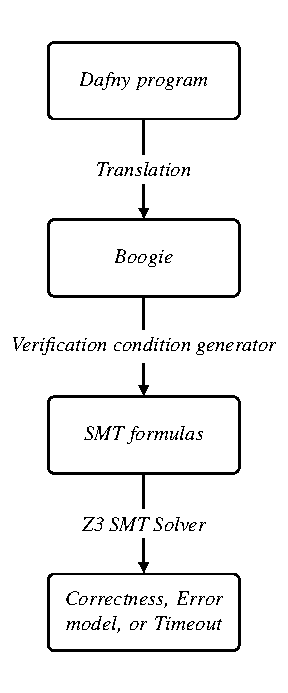
\includegraphics[width=\textwidth,keepaspectratio]{fig_dafny}
\caption[Overview of Dafny implementation and verification workflow]{
A (simplified) overview of Dafny implementation and verification workflow.
\enquote{A well-designed language and verifier, plus a great SMT solver, go a long way.} -- \textcite{leino2010b}.}
\label{fig:dfy-flow}
\end{figure}

\paragraph*{Technical overview.}
Dafny is a hybrid language, influenced by \ndx{Java} and \ndx{C\#}.
It has both functional and object-oriented features;
including: curly-bracket block-style, (mathematical) functions, and inductive and co-inductive\index{coinduction} data types.
The programming constructs include loops, \pr|if|-statements, arrays, classes and methods;
variables, types, generics, lambdas, inheritance, \etc~\cite{dafnydoc}
The real power of \ndx{Dafny} comes from the ability to annotate methods to specify their behavior.
For verification tasks, the idea is to define specifications and write proofs aside the implementation, in \ndx{deductive verification}-style.
The built-in verification constructs include pre- and postconditions;
loop invariants, termination metrics, lemmas, and \ndx{ghost construct}s\footnote{
A \emph{ghost} is any construct that is used for verification only; they are erased during compilation~\cite[p. 19]{leino2023}.}.
This language design enables writing functionally-correct verified programs fully in \ndx{Dafny}~\cite{leino2023}.
Dafny programs can be compiled to various target languages, like \ndx{C\#}, \ndx{Java}, and \ndx{Go}~\cite{dafnydoc}.

Dafny has an associated static program verifier.
The role of the verifier is to check a program's specification constructs\footnote{These are Eiffel-like contracts from~\cite{meyer1988}.}.
As visualized by the chart in~\autoref{fig:dafny-auto} (inspired by~\cite{leino2010b}), the built-in verifier in Dafny adds a high degree of automation.
The verifier resolves many low-level proof steps.
For example, if we wanted to prove the lemma of~\autoref{lst:rocq-basic} in Dafny, the verifier succeeds at discharging the proof obligations automatically -- see \pr|Add0Left| in~\autoref{fig:dafny-use}.

\begin{figure}[ht]
\centering
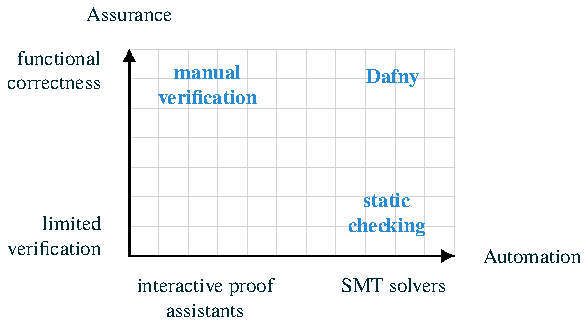
\includegraphics[width=.7\textwidth,keepaspectratio]{fig_chart}
\caption[Automation degree chart]{Automation degree.}
\label{fig:dafny-auto}
\end{figure}

\begin{figure}[p]
\begin{center}
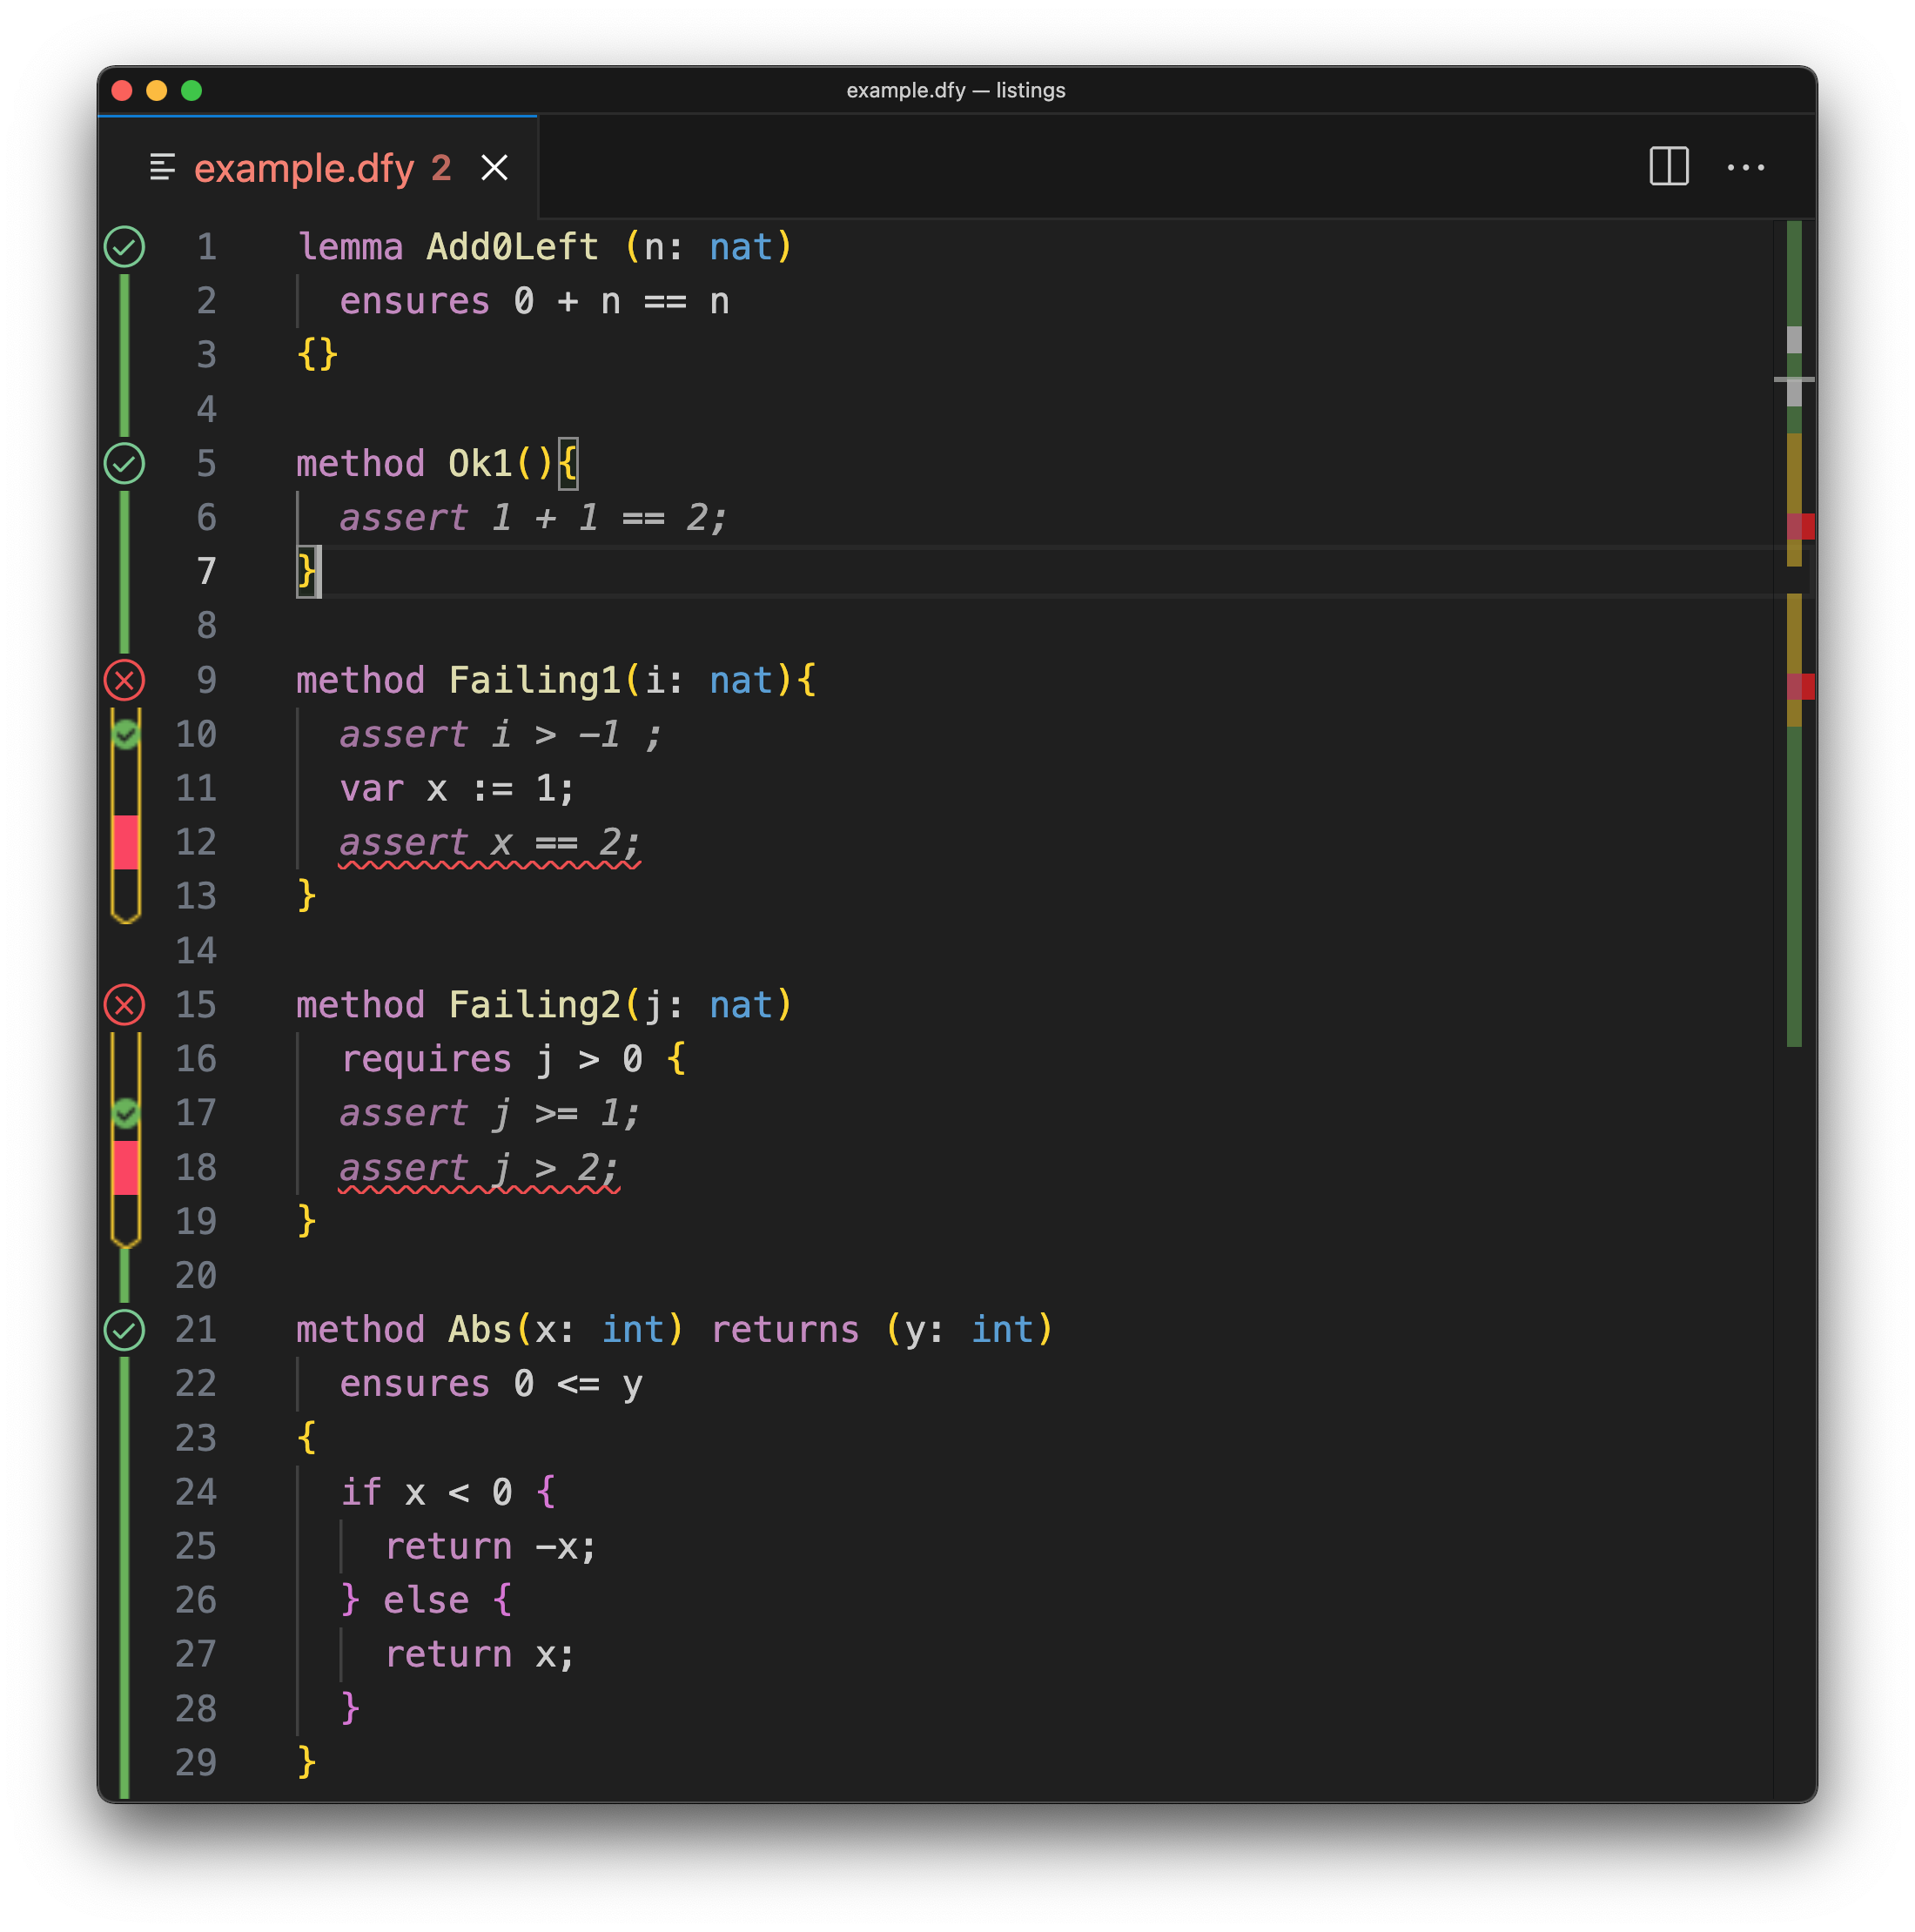
\includegraphics[width=\textwidth,keepaspectratio]{fig_vs1}
\end{center}
\caption[Dafny running in Visual Studio Code]{
The Dafny verifier checking Dafny code (running in Visual Studio Code).
A big green check{ }{ }\circledb[dafnyok]{\faCheck}{ }means the verifier succeeds at proving the corresponding program construct.
A big red cross{ }{ }\circledb[dafnyno]{\scalebox{1.25}{\faTimes}}{ }identifies program constructs that fail to verify completely, even if some inner declarations succeed.
A green filled check {\color{dafnyok}{\scalebox{.8}{\faCheckCircle}}} means the verifier succeeds at the proof obligation at the corresponding line.
The verification fails at declarations marked with a red block \langclr{dafnyred} and\;\;\uwave{squiggly underline}{}.
}\label{fig:dafny-use}
\end{figure}

A program accepted by the Dafny verifier is guaranteed to be totally correct, \ie it terminates and satisfies its specification.
During program development and when given a candidate specification, the verifier runs automatically on code edits, as shown in~\autoref{fig:dafny-use}.
The engineer receives immediate feedback on their verification efforts.
When Dafny verifier fails, the user must annotate the program with additional guidance---assertions, pre-conditions, lemmas, \etc---to assist the verifier, until the verification succeeds.
Logical contradictions, like the ones raised in~\autoref{fig:dafny-use}, will obviously never succeed.
The verifier helps to catch such errors early in the program development phase.

\paragraph*{Proof style.}
In Dafny, proofs are developed in \enquote{top-down} style.
This allows the developer to focus on the proof architecture before the detailed proof steps.
To this end, Dafny provides the constructs of \pr|assume| statements, \ie assertions without a proof;
and ghost methods, \ie lemmas that are not yet proven.
Obviously, the proof is not complete until these temporary constructs have been replaced with concrete proofs.
However, they are useful for facilitating the proof development.

\paragraph*{Boogie.}
{Boogie}~\cite{leino2008}\index{Boogie} is an intermediate verification language, used in the verification workflow of Dafny programs (\cf~\autoref{fig:dfy-flow}).
More generally, Boogie is an open source modeling language and a verification tool for sequential and concurrent programs, and distributed systems~\cite{boogie}.
It provides a layer on which to build program verifiers\footnote{
Several program verifies are built on Boogie, for example Dafny, Chalice, Spec\#, and Move~\cite{boogie}.}.
When viewed as a verification tool, Boogie takes as input a program written in the Boogie language.
Then, the tool infers invariants, generates verification conditions, and passes them to an SMT solver.
The default SMT solver is Z3~\cite{demoura2008}.

\paragraph*{Applications of Dafny.}
Dafny is a mature, industry-grade tool for program verification.
It has been used in research projects, industrial applications, verification projects, and in teaching formal methods.
Among the hallmark results, the AWS authorization engine---that handles 1 billion API calls per second~\cite{wagner2024}---is verified in Dafny~\cite{chakarov2025}.

\subsubsection{Tool Comparison by Light Examples}
\label{subsubsec:sm-tool-examples}

This section covers two verification tasks that are suitable for paper presentation while illustrating differences between the formal proof techniques.
To match the dissertation theme, the examples are about program proofs.
However, proving programs is only a subset of the general utility of these tools;
refer to \autoref{tab:rocq-results} for more cases.

\paragraph{Program Equivalence}

\autoref{lst:intro} in the introduction showed two programs with a claim that the programs are equivalent.
Equivalence means that, for all inputs, they compute the same result.
With manual inspection, one can become reasonably convinced that the claim is true.
However, such inspection provides only weak informal guarantees.
We can do better -- we now have the tools to prove formally the claim about equivalence.

\begin{center}
%\begin{minipage}{\textwidth}
\captionsetup{type=lstlisting}
\rocqinputlisting[breakable][firstline=176]{equiv.v}
\captionof{lstlisting}[A Rocq proof of program equivalence]{A Rocq proof of program equivalence (theorem only).
The full proof with the programming language syntax, semantics, and notations is about 200 LOC.}
\label{lst:eq-proof}
%\end{minipage}
\end{center}

\subparagraph*{The Rocq proof explained.}
The Rocq theorem (L5--8) makes explicit that the equivalence holds when
\pr|X| and \pr|Y| are arithmetic expressions that evaluate to a \(\mathbb{N}\); \pr|Z| is a variable, and \pr|b| has value \(0\) or \(1\).
The precise programming language semantics are defined as part of the full proof.
The property of \emph{equivalence} is defined as a proposition (L1--3).
Informally, two programs (commands, \pr|c1| and \pr|c2|) are equivalent
iff they start execution in the same state (\pr|st|) and reach the same final state (\pr|st'|), for all states.
Although program termination is not guaranteed by this specification,
the state-based definition requires that equivalent programs must agree on divergence.
That is, if one program diverges, the other must diverge also.
The actual proof steps, in L9--23, show how to establish equivalence of the programs in~\autoref{lst:intro}.
At a high level, the proof proceeds as follows.
First, we split the bijection (\( \leftrightarrow \)) to inspect both directions of the equivalence.
Next, we substitute \pr|b| with concrete values, which creates additional subcases.
Some of these cases are contradictory and resolved easily by the \pr|discriminate| tactic (L13).
The proof concludes by applying algebra on the multiplication operations;
that is then sufficient to prove equivalence (L16, L22).
Without technical familiarity, the steps may not be easily readable from the tactics.
Yet, as for all mechanized proofs, it is possible for everyone to check the proof by compiling it.
Further, it is possible to inspect the proof steps in an editor or IDE\footnote{
Since the proof includes much symmetry and automation,
the proof needs some editing to reduce the automation before inspecting the intermediate steps.}.
Thus, a mechanized proof lifts the observer's need to understand the details of the proof to \enquote{just} understanding the stated theorem, and trusting the proof assistant with checking it.

\begin{center}
\begin{minipage}{\textwidth}
\captionsetup{type=lstlisting}
\dafnyinputlisting[][]{equiv.dfy}
\captionof{lstlisting}[Proof of program equivalence in Dafny]{
Program equivalence verified in Dafny (complete).
The listing includes a subtype definition of \pr|bit| that does not occur in the Rocq version.}
\label{lst:eq-dafny}
\end{minipage}
\end{center}

\subparagraph*{The Dafny verification explained.}
The Dafny version in~\autoref{lst:eq-dafny} contains the full details of the proof.
To make life a bit more interesting, it defines a subtype of \pr|bit|.
Alternatively, the restriction on the values of \pr|b| could be stated as a precondition.
Next, the listing shows a \pr|function| and a \pr|method|.
A \emph{method} in Dafny is a piece of imperative executable code, which can have all sorts of statements in its body.
The term \emph{function} is reserved for constructs that can be used directly in specifications.
Unlike a method, a function body must consist of exactly one expression, and it returns a value.
For the ways the two programs were originally written and for demonstration,
it makes sense to define the programs as a function and a method\footnote{
Specifying two methods is also possible, the proof will just look different.}.
Because \pr|Program2| is a function, it can be used in the specification condition of \pr|Program1|.
The \pr|ensures| clause says the value computed by \pr|Program1| is exactly equal to that
computed by \pr|Program2|, for all arguments.
The equivalence holds in both directions.
Because the equivalence is generally easy to show, the verifier succeed without additional lemmas,
which proves the equivalence claim.

\paragraph{Formally verified leftpad.}
Leftpad is a string manipulation function.
It pads a string, using a specified character, up to a specified length.
The padding character is applied to the left side of the string, as a prefix, hence the name.
\autoref{lst:leftpad} shows examples of leftpad behavior.

\begin{center}
\captionsetup{type=lstlisting}
\begin{minipage}{\textwidth}
\begin{minipage}{.45\textwidth}
\cmdinputlisting{leftpad.cmd}
\end{minipage}%
\hfill\(\Rightarrow\)\hfill%
\begin{minipage}{.45\textwidth}
\outinputlisting[][numbers=none]{leftpad.output}
\end{minipage}
\end{minipage}
\captionof{lstlisting}[Leftpad in action]{Leftpad in action.}
\label{lst:leftpad}
\end{center}

The \href{https://github.com/hwayne/lets-prove-leftpad}{\enquote{Let's Prove Leftpad}}~\cite{leftpad} is public challenge project initiated by Hillel Wayne.
The idea is to put different verification tools and proof techniques to test by using them to prove leftpad.
At the time of writing this (April 2025), the repository contains 29 variants of leftpad proofs.
The challenge is interesting, because a leftpad proof is small enough to be accessible without formal methods background, yet complex enough to differentiate the proof techniques.
The leftpad implementation is simple, but the formal specification is surprisingly tricky.
A formal proof requires showing that the following three specification conditions hold.

\begin{enumerate}
\item Given pad length \(n\) and a string \pr|str|, the output length is \(\max(n, \text{len}(\prm{str}))\).
\item The output prefix is padding characters and nothing but padding characters.
\item The suffix of the output is the original string \pr|str|.
\end{enumerate}

Listings~\autoref{lst:rocq-leftpad}--\ref{lst:leftdfy} show the complete implementations and proofs of leftpad in Rocq;
the SSReflect of the Mathematical Components library, and Dafny.
The proofs come from the \enquote{Let's Prove Leftpad} project repository~\cite{leftpad}.
They were originally crafted by Ezra Cooper (Rocq), Anton Trunov (SSReflect), and Hillel Wayne (Dafny).
The proofs are modified for paper presentation and to resolve language updates, with the Rocq proof modified heavily from its original form.
The padding character is represented as \pr|c|, the pad length is \pr|n|, and the input \enquote{string}\footnote{
    None of the proofs actually refer to \emph{string} type, though one uses a sequence of characters.} is \pr|s|.
Each version includes an implementation and a proof to show that the implementation satisfies the specification.

\begin{center}
\captionsetup{type=lstlisting}
\rocqinputlisting[breakable][firstline=2]{leftpad.v}
\captionof{lstlisting}[Leftpad in Rocq]{Leftpad in Rocq.}
\label{lst:rocq-leftpad}
\end{center}

\subparagraph*{Leftpad in Rocq.}
The Rocq proof of leftpad is shown in~\autoref{lst:rocq-leftpad}.
The leftpad implementation (at L27--28) is intuitive --
it works by concatenating \(n - \text{length}(\prm{s})\) count of  symbols \pr|c| with \pr|s|.
Since the proof compiles successfully, we also know the leftpad implementation is guaranteed to terminate.
In the proof, the key idea is that it is possible to cut the concatenated string to a prefix and suffix, at index \(m\).
The specification is then proved \wrt the prefix and suffix, and the concatenated length.
Proving the theorem requires introducing the supporting definitions and lemmas of L6--25.

\subparagraph*{Leftpad in SSReflect.}
The Mathematical Components library does not contain definitions of string or character types,
which is why~\autoref{lst:mathcomp-leftpad} is generalized to a parametric type \pr|T|.
The leftpad implementation, at L8--9, is functionally the same as in~\autoref{lst:rocq-leftpad},
only expressed in the style of mathcomp.
The three lemmas that follow prove the specification.
The first lemma \pr|length_max_spec| matches the Rocq version in~\autoref{lst:rocq-leftpad},
but the prefix and suffix proofs are achieved differently.
The latter rely on a random access function \pr|nth| that returns the \(i\)-th element in a sequence
(numbered from 0), or the \pr|def| element, if the sequence contains fewer than \(i+1\) elements.
In the proofs, the imported libraries provide much assistance.
In SSReflect, it is common for simple proofs to require only rewrites, while \enquote{interesting proofs} appear visually longer.
The leftpad proof is simple since it requires only rewrites, and those rewrites are defined by the library.
The tactics naming convention is a design feature of the Mathematical Components library.
The naming eases locating proofs;
otherwise, one must search the proofs database.

\begin{center}
\captionsetup{type=lstlisting}
\begin{minipage}{\linewidth}
\mathcompinputlisting[][firstline=2]{leftpad_ssrefl.v}
\captionof{lstlisting}[Leftpad in SSReflect proof language]{Leftpad in the SSReflect proof language of the Mathematical Components library.}
\label{lst:mathcomp-leftpad}
\end{minipage}
\end{center}

\begin{center}
\begin{minipage}{\linewidth}
\captionsetup{type=lstlisting}
\dafnyinputlisting[][]{leftpad.dfy}
\captionof{lstlisting}[Leftpad formally verified in Dafny]{Formally verified leftpad in Dafny.}
\label{lst:leftdfy}
\end{minipage}
\end{center}

\subparagraph*{Leftpad in Dafny.}
In Dafny, the specifications are \enquote{embedded} with the implementation.
To make the \autoref{lst:leftdfy} standalone, the \pr|Max| function is defined inline.
The three specification conditions correspond (in order) to the \pr|ensures| clauses.
The same conditions re-appear as loop invariants at L14--16.
The \pr|invariant| clauses are necessary to convince the verifier that the conditions are preserved over iteration of the loop.
Enhancing the \pr|while| loop is sufficient for the verifier to succeed at proving the implementation meets the specification.
There's one more proof obligation for loops, which is to show termination.
The \pr|decreases| clause proves termination, which established total correctness of the \pr|LeftPad| method.

\subparagraph*{Observable differences.}
Although the leftpad behavior is consistently the same,
the examples show different styles of implementation and varying approaches to proving that the implementation is \emph{totally correct}.
The Rocq prover is very flexible in supporting various kinds of proofs and enables fine-grained control over the specification.
The \enquote{built-in} specification style of Dafny -- with pre-and postconditions, invariants, and termination -- is natural and powerful for proving programs.
Much of the power comes from automatic decision procedures, but can be challenging to debug if the verification fails.
In general, it is important to understand the mechanics of the selected tool, since a tool choice greatly influences the proof style and built-in capabilities.

\subsubsection{The Moscow Problem}
\label{subsec:moscow}

The next problem is a more involved and interesting for formal techniques and logic.
The problem was presented to me by Natarajan Shankar under the name \enquote{the Moscow problem}.
Although it is too simple for research, it is also too fascinating to be left in obscurity.
Therefore, it appears here, in my dissertation.

\paragraph*{Problem Description.}
Assume there are three people, \(\mathsf{A}\), \(\mathsf{B}\), and \(\mathsf{C}\)\@.
Seven natural numbers in 1--7 are distributed randomly among the people.
\(\mathsf{A}\) gets 1 number, and \(\mathsf{B}\) and \(\mathsf{C}\) get 3 numbers each.
The numbers are distinct, \ie no two people hold the same number;
and the distribution is secret, \ie it is unknown who holds what numbers.
The challenge is to design a message exchange that meets the following requirements.

\begin{enumerate}
\item \(\mathsf{B}\) sends one message to \(\mathsf{C}\) and from that message, \(\mathsf{C}\) knows what numbers everyone holds.
      (And similarly in reverse: \(\mathsf{C}\) sends one message to \(\mathsf{B}\)\ldots).
\item \(\mathsf{A}\) observes the messages but \(\mathsf{A}\) \enquote{does not learning anything}.
      In other words, \(\mathsf{A}\) cannot determine who holds what numbers based on the observed messages.
\end{enumerate}

Messages are exchanged in plain text and \(\mathsf{A}\) is aware of the mechanics of the exchange protocol.
The Moscow problem is to design a technique that meets the requirements.
The following solution is what I have developed in response to the problem.

\paragraph*{Informal Solution.}
Starting with a claim: it is sufficient to achieve the desired system with a message exchange where the message value is a single digit in 1--7.

The exchange is symmetric.
Therefore, instead of referring to \(\mathsf{B}\) and \(\mathsf{C}\), we say \emph{sender} and \emph{receiver}.
The sender calculates the exchanged value (the single digit) using only the numbers they hold.
The receiver calculates---using the single digit and number they holds---the number \emph{held by \(\mathsf{A}\)}.
Finally, the receiver deduces the numbers held by the sender.
There are three important functions.
\begin{enumerate}
\item \emph{Send} function that calculates the exchanged digit.
\item \emph{Receive} function that calculates number held by \(\mathsf{A}\).
\item \emph{Recover} function that deduces values held by the sender.
\end{enumerate}

The functions are defined as follows.
The universe is \(U = \{ x \mid 1 \leq x \leq 7 \}\).
Letting \(X\) be a set of numbers in \(U\), the numbers \enquote{outside} \(X\) are defined by
the set complement \(\overline{X} = U - X\).
Letting \(y\) be a number in \(U\), we \emph{encode} a value by
\[\text{E}(X, y) =
\begin{cases}
7, & \text{if } \Sigma\,\overline{X} + y\pmod{7} = 0 \\
\Sigma\,\overline{X} + y\pmod{7}, & \text{otherwise}
\end{cases}\]
Letting the set of numbers held by the \emph{sender} (\resp \emph{receiver}) be \(X_s\) (\resp \(X_r\)),
we define the function \emph{send} as \(\text{S}(X_s) = \text{E}(X_s, 7)\).
The send function produces the exchanged message value \(m\) that is observable to everyone.
The function \emph{receive} is \(\text{R}(X_r,m) = \text{E}(X_r, m)\),
and it produces the number held by \(\mathsf{A}\), denoted as \(a\).
The receiver calculates numbers held by the sender using the \emph{recover} function \(\text{Rec}(X_r, a) = U - X_r - a\).

\paragraph{Formal proof.}
The interesting bit is showing that the solution meets the specification.
The solution is provable in the Rocq prover.
We define first the messaging functions as shown in~\autoref{lst:moscow-fun}.

\begin{center}
\begin{minipage}{\textwidth}
\captionsetup{type=lstlisting}
\mathcompinputlisting[][firstline=28,lastline=37]{moscow.v}
\captionof{lstlisting}[Moscow messaging functions]{Implementation of the messaging functions. The \pr|t| is a triple of natural numbers and
\pr|T3| converts an arbitrary-length sequence (back) to a triple.}
\label{lst:moscow-fun}
\end{minipage}
\end{center}

The message exchange requirements are defined by two lemmas.
First, \enquote{\(\mathsf{C}\) (\resp \(\mathsf{B}\)) learns everything from one message} is stated formally as shown in~\autoref{lst:lemma-1}.
The lemmas essentially says the receiver (\pr|R|) recovers (some permutation) of numbers that match exactly those held by the sender (\pr|S|).
The \pr|send S| is the value of the exchanged message.

\begin{center}
\begin{minipage}{\textwidth}
\captionsetup{type=lstlisting}
\mathcompinputlisting[][]{lemma1.v}
\captionof{lstlisting}[Receiver knows sender]{First requirement formally -- receiver learns the numbers held by sender.}
\label{lst:lemma-1}
\end{minipage}
\end{center}

An \emph{allocation} (type \pr|alloc|) represents a distribution of numbers in \(U\)
between \(\mathsf{A}\), \(\mathsf{B}\), and \(\mathsf{C}\).
The second criterion is that \enquote{\(\mathsf{A}\) does not learn anything}.
We formalize this in~\autoref{lst:lemma-2}.
The lemma says, for every allocation of numbers and after observing both message exchanges between \(\mathsf{B}\) and \(\mathsf{C}\),
\(\mathsf{A}\) has \emph{insufficient information}
to determine with certainty what numbers everyone is holding.
In other words, any observed exchanges can be explained by at least two different allocations,
because there exists an alternate (different) \pr|alloc2| that explains the observations of \(\mathsf{A}\).

\begin{center}
\begin{minipage}{\textwidth}
\captionsetup{type=lstlisting}
\mathcompinputlisting{lemma2.v}
\captionof{lstlisting}[Person A cannot recover the allocation]
{Second requirement formally -- \(\mathsf{A}\) does not learn anything.}
\label{lst:lemma-2}
\end{minipage}
\end{center}

A complete machine-checkable implementation and a proof is available in the dissertation artifact
(\cf~\aref{app:sec:artifacts} in \pr|code/moscow.v|).
To machine-check the proof, we compile the file in a terminal following the instructions of the artifact readme.
The expectation is that the proof should compile without errors (it does not print any terminal output).

Compilation of the proof also runs an extraction routine.
The extraction generates a certified \ndx{OCaml} program (\pr|message.ml|) from the messaging functions implemented in \ndx{SSReflect}.
Another program---\pr|exchange.ml|, also in the dissertation artifact (\cf~\autoref{tab:pub-artifacts})---is a {driver} for running the certified program.
The driver uses the certified program to perform a message exchange when run as shown in~\autoref{lst:run-exchange}.

\begin{center}
\captionsetup{type=lstlisting}
\begin{minipage}{\textwidth}
\cmdinputlisting{exchange.cmd}
\outinputlisting[][firstline=2,lastline=3]{exchange.output}
\end{minipage}
\captionof{lstlisting}[Running a certified message exchange]
{Running a certified message exchange. In this scenario, \(\mathsf{A}\) holds
the number 2, and everyone observes the messages \enquote{4} and \enquote{5}.
This information is not enough for \(\mathsf{A}\) to learn what numbers
\(\mathsf{B}\) (\resp \(\mathsf{C}\)) is holding. However, by the end of the
exchange, \(\mathsf{B}\) and \(\mathsf{C}\) are fully informed.}
\label{lst:run-exchange}
\end{center}

The presented moscow problem solution could be adjusted to a universe of \([0,
6]\) with a small change.
However, it is unknown whether other modifications---\eg larger set of numbers,
different allocations, or more people---could be added.

\subsubsection{Connecting Formal Methods and ICC}
\label{subsubsec:icc-formally}

There are several ways to relate complexity theory and formal methods. Since
they are founded on programming languages, ICC systems are potentially highly
suitable for formal reasoning (\cf~\textcite{cpierce20222} for a starting
point). A particularly strong motivator is that ICC systems yield more natural
definitions and proofs of central results than classic \ndx{complexity
theory}~\cite{kristiansen2017}.

Formalization of a theory requires significant time and effort.
However, the effort of formalizing ICC results is justified, based on the
continued demonstrated relevance of ICC results -- \cf~\autoref{tab:icc-results},
absence of \emph{formal} proofs among those results, and
maturity of formalization techniques and tools.

\paragraph*{Existing results in formally verified complexity.}
There exists a (small) collection of result formalizing classic \ndx{complexity
theory} (\cf~\autoref{subsec:coqpl-related}). For example,
\ndx{Universal Turing Machine}s~\cite{forster2020}, the
\(\mathcal{O}\)-notation\symbo{bigo}~\cite{gueneau2018},
and the \ndx{Cook-Levin theorem}~\cite{gaher2021}\footnote{
The Cook-Levin theorem states that Boolean SAT is NP-Complete\ccxi{np}~\cite{cook1971, levin1973}.}
have been formalized previously.

Among programming language-based approaches, the type system of~\cite{crary2000}
is notable. The type system assigns a \enquote{virtual clock} to a program.
Then, a compile-time check aims to verity that the clock does not expire.
Although this provides an automatic method for certifying resource usage, the
theory is not formalized mechanically. The cost-aware logical framework
\ndx{Calf}~\cite{niu2022}---and its extension
\ndx{Decalf}~\cite{grodin2024}---is similarly a type system-based approach for
functional programs. Calf embeds, thought types, the amortized
costs\index{amortization} of computation. It also uses clocks, where the clocks
record the recursion depth, to ensure termination of programs in total type
theory. Then, if a program can be typed, the Calf system ensures that the
program satisfies the specified resource bound. The type system definitions is
\href{https://github.com/HarrisonGrodin/agda-calf}{formalized in
\ndx{Agda}}~\cite{grodin2023}.

Among works of implicit computational complexity, the hallmark result of
Bellantoni and Cook (\ndx{safe recursion}~\cf{safe-rec}) was formalized
in~\textcite{heraud2011}. The Rocq library
\href{https://github.com/davidnowak/cecoa}{Cecoa}{\ndx{Cecoa}} enables proving
that a user-defined function is polytime computable~\cite{feree2018}. It is
based on \ndx{quasi-interpretation}s of~\textcite{marion2000} and extends the
Bellantoni and Cook formalization. The \ndx{Cecoa} library is between complexity
theory and program analysis. However, it is not an automatic program analyzer,
since user effort is needed to establish the complexity result.

To the best of our knowledge, no formalized automatic resource analyzer exists.
The closest to the goal are the analyzers \ndx{C4B} and \ndx{Pastis}
(\cf~\autoref{resource-analysis-tools}), that produce \emph{proof certificates}
for the bounds they compute. The analysis technique--that is based on
\ndx{automatic amortized resource analysis}
(cf~\autoref{resource-analysis})---is founded on inference rules. After program
analysis, the derivation trees are translated to machine-checkable proofs. The
proof certificates are produced via a support library that complements the core
analysis. However, the analysis {technique} is not proven correct.

\paragraph*{From implicit complexity towards formal methods.}
There is much room to improve the state-of-the-art in formal reasoning about
complexity, both in terms of theory and analysis. Implicit computational
complexity presents a potential avenue toward advancement.

Given the demonstrated applications and familiarity, the flow calculus of
mwp-bounds\index{mwp-calculus} is an appealing target for formalization. An
important step is proving formally the mwp-calculus soundness
theorem\index{soundness of mwp-calculus} (\autoref{mwp-soundness}). The aim has
multiple sources of support. First, the paper proofs are available
in~\cite{jones2009}. Second, our confidence in the correctness of the theory is
high. If a problem existed, it likely would have already surfaced in the prior
projects.

However, converting the mwp-calculus to a formal proof poses various technical
challenges. For example, how to model the mathematical framework of the flow
calculus, and converting the proofs between logical formalisms, from set theory
to type theory. Moreover, a proof of the original flow calculus would not extend
to the \textsc{mwp}$^\infty$\symbo{mwpi}-calculus variant, that is used in
program analysis. Yet, starting with the core mwp-calculus and paper proofs is a
solid strategy toward formalizing complexity. The result would extend broadly to
all programs that share the same imperative core. This project idea is discussed
in~\autoref{sec:mwp-calc-formal}.

It is important to note the utility of implicit computational complexity is not
limited to formalizing complexity results. Another perspective is to use ICC
systems in assisting formal methods tools in program verification efforts. This
is the motivating idea in the manuscript of~\autoref{sec:postcond}. The central
idea is that the inferred mwp-bounds can aid the discovery of verification
conditions in \ndx{Dafny}-style deductive verification.
